% Template for Cogsci submission with R Markdown

% Stuff changed from original Markdown PLOS Template
\documentclass[10pt, letterpaper]{article}

\usepackage{cogsci}
\usepackage{pslatex}
\usepackage{float}
\usepackage{caption}

% amsmath package, useful for mathematical formulas
\usepackage{amsmath}

% amssymb package, useful for mathematical symbols
\usepackage{amssymb}

% hyperref package, useful for hyperlinks
\usepackage{hyperref}

% graphicx package, useful for including eps and pdf graphics
% include graphics with the command \includegraphics
\usepackage{graphicx}

% Sweave(-like)
\usepackage{fancyvrb}
\DefineVerbatimEnvironment{Sinput}{Verbatim}{fontshape=sl}
\DefineVerbatimEnvironment{Soutput}{Verbatim}{}
\DefineVerbatimEnvironment{Scode}{Verbatim}{fontshape=sl}
\newenvironment{Schunk}{}{}
\DefineVerbatimEnvironment{Code}{Verbatim}{}
\DefineVerbatimEnvironment{CodeInput}{Verbatim}{fontshape=sl}
\DefineVerbatimEnvironment{CodeOutput}{Verbatim}{}
\newenvironment{CodeChunk}{}{}

% cite package, to clean up citations in the main text. Do not remove.
\usepackage{apacite}

% KM added 1/4/18 to allow control of blind submission


\usepackage{color}

% Use doublespacing - comment out for single spacing
%\usepackage{setspace}
%\doublespacing


% % Text layout
% \topmargin 0.0cm
% \oddsidemargin 0.5cm
% \evensidemargin 0.5cm
% \textwidth 16cm
% \textheight 21cm

\title{How to Make a Proceedings Paper Submission}

\usepackage{booktabs}
\usepackage{longtable}
\usepackage{array}
\usepackage{multirow}
\usepackage{wrapfig}
\usepackage{float}
\usepackage{colortbl}
\usepackage{pdflscape}
\usepackage{tabu}
\usepackage{threeparttable}
\usepackage{threeparttablex}
\usepackage[normalem]{ulem}
\usepackage{makecell}
\usepackage{xcolor}

\author{{\large \bf Morton Ann Gernsbacher (MAG@Macc.Wisc.Edu)} \\ Department of Psychology, 1202 W. Johnson Street \\ Madison, WI 53706 USA \AND {\large \bf Sharon J.~Derry (SDJ@Macc.Wisc.Edu)} \\ Department of Educational Psychology, 1025 W. Johnson Street \\ Madison, WI 53706 USA}

\newlength{\cslhangindent}
\setlength{\cslhangindent}{1.5em}
\newenvironment{CSLReferences}%
  {}%
  {\par}

\begin{document}

\maketitle

\begin{abstract}
Include no author information in the initial submission, to facilitate
blind review. The abstract should be one paragraph, indented 1/8 inch on
both sides, in 9\textasciitilde point font with single spacing. The
heading `Abstract' should be 10\textasciitilde point, bold, centered,
with one line of space below it. This one-paragraph abstract section is
required only for standard six page proceedings papers. Following the
abstract should be a blank line, followed by the header `Keywords' and a
list of descriptive keywords separated by semicolons, all in
9\textasciitilde point font, as shown below.

\textbf{Keywords:}
Add your choice of indexing terms or keywords; kindly use a semi-colon;
between each term.
\end{abstract}

\hypertarget{introduction}{%
\section{Introduction}\label{introduction}}

Whether to keep looking at a current target of attention is one of the
most fundamental decisions we make, whether we are trying to find our
way in a busy street or swiping through TikTok. Even young infants
constantly decide whether to keep looking or move on. In fact, infant
research has long capitalized on infants' ability to endogenously
control their attention, making inferences about infants' learning and
mental representations from changes in their looking duration (Aslin,
2007; Sim \& Xu, 2019). In a typical experiment, infants decrease their
looking duration upon seeing the same stimulus repeatedly
(i.e.~habituation). Then, infants' often recover interest when seeing a
novel stimulus (i.e.~dishabituation). While these phenomena are
well-documented, the mechanisms underlying them remain poorly
understood. A better understanding of what shapes habituation and
dishabituation is of both methodological and theoretical significance.
Methodologically, assumptions about habituation and dishabituation
underpin many other claims about infants' cognitive repertoire (Paulus,
2022; Tafreshi, Thompson, \& Racine, 2014). Theoretically, it would shed
light on infants' active role in shaping their own learning and reveal
principles that guide human information-seeking behavior in general (Raz
\& Saxe, 2020; Smith, Jayaraman, Clerkin, \& Yu, 2018). Here we provide
a model of the basic decision faced by infants in a standard looking
paradigm. To do so, we model looking as rational active selection of
noisy perceptual samples for learning. Our goal is to describe the
proximal computations that could underlie the moment-to-moment decision
of whether to keep looking at the current stimulus, or look away to find
a different stimulus.

Classical theory of infant looking posits that infants look at stimuli
in order to learn or encode them, so the dynamics of looking time are
driven by the dynamics of learning (Hunter \& Ames, 1988). The more an
infant has already been exposed to a stimulus, the less they have to
learn about it (i.e.~increasing exposure time should decrease looking).
The more complicated a stimulus is, the more that would still remain to
learn after any given exposure time (i.e.~increasing complexity should
increase looking). Individual infants may also differ in how long it
takes them to learn a given stimulus (e.g.~older infants may habituate
after less exposure. Although this theory is influential, little
empirical work has examined it systematically (for exceptions, see
Hunter, Ames, \& Koopman, 1983) and the lack of quantitative details in
the theory has made it impossible to offer precise predictions.

In contrast to the classical verbal theory, recent work has attempted to
describe infants' looking behaviors through computational modeling. In
pioneering work, Kidd, Piantadosi, \& Aslin (2012) developed a paradigm
in which infants are shown sequences of events. Infants' look-away
probabilities away from the stimuli are compared with surprisal, a
measure of information content, derived from a rational learner model
that keeps track of the probabilities of each event. The study shows
that infants' pay most attention to event sequences that are neither too
high nor too low in surprisal, resulting in a `Goldilocks' effect of
attention. A recent study by Poli, Serino, Mars, \& Hunnius (2020)
offered an alternative linking hypothesis between the model and
behavior: the study used a similar paradigm and model to show that
infants' looking time can be predicted by `learning progress,'
formalized as the Kullback-Leibler (KL) divergence between the the
model's knowledge before and after each stimulus. These attempts to
connect information theoretic measures to infants' looking time resonate
with previous literature on information foraging that postulates human
exploratory behaviors are driven by maximizing information gain (Hills,
Todd, \& Goldstone, 2008; Pirolli \& Card, 1999) as well as the emerging
literature on curiosity in developmental robotics and reinforcement
learning (Haber, Mrowca, Fei-Fei, \& Yamins, 2018; Oudeyer, Kaplan, \&
Hafner, 2007), as well as information foraging . Curiosity-driven
artificial agents' exploratory behaviors can be guided by optimizing
expected information gain (EIG), a measurement that has been shown to be
related to curiosity-driven learning in human children and adults (e.g.,
Liquin, Callaway, \& Lombrozo, 2021).

However, there are several limitations to the existing models. First,
current models do not capture the noisy nature of perceptual learning
(Callaway, Rangel, \& Griffiths, 2021; Kersten, Mamassian, \& Yuille,
2004). That is, the models were assumed to acquire perfect
representation of each event in the sequence. This assumption leads to
the second limitation: While surprisal and KL-divergence have been shown
to correlate with infants' looking behaviors, current models do not
provide an account of how these measurements might be linked
mechanistically to infants' behavior. Previous models show that infants
might be sensitive to the information-theoretic variability in their
learning environment, but they do not provide an account of how they are
related to infants' real-time sampling behavior. Finally, the event
sequence paradigm used to evaluate these models are not representative
of classical infant looking time paradigms. As the key phenomena
described in the Hunter \& Ames (1988) theory were not captured, the
extent to which we can extrapolate current model fits to behavior in a
typical looking time experiment remains limited.

Here we present steps toward overcoming these limitations. Our goal is
to provide a unifying quantitative account of looking behaviors as
arising from optimal decision-making over noisy perceptual
representations (Bitzer, Park, Blankenburg, \& Kiebel, 2014; Callaway et
al., 2021). To do so, we present the ``rational action, noisy choice for
habituation'' (RANCH) model. RANCH works by a) accumulating noisy
samples from the stimulus, and b) rationally choosing what to look at
using different information-theoretic linking hypotheses (surprisal,
KL-divergence, and EIG). Finally, we evaluate RANCH with adult looking
time data collected from a paradigm that captures habituation,
dishabituation, and complexity effects.

\hypertarget{model}{%
\section{Model}\label{model}}

We reasoned that, at its simplest, habituation occurs when each
repetition of a stimulus refines the representation of a concept until
repetitions become ineffectual. Dishabituation then occurs when a
stimulus deviates from the concept learned during habituation. We
therefore formalized the learning problem that participants face in a
simple habituation experiment as a form of Bayesian concept learning
(Goodman, Tenenbaum, Feldman, \& Griffiths, 2008; Tenenbaum, 1999).
Figure 1. shows the plate diagram illustrating the model's architecture.

\hypertarget{learning}{%
\subsection{Learning}\label{learning}}

The goal is to learn a concept \(\theta\), which is a set of
probabilities for independent binary features \(\theta_{1,2,..,n}\),
where n is the number of features. \(\theta\) in turn generates
exemplars \(y\): instantiations of \(\bar{\theta}\), where each feature
\(y_{1,2,..,n}\) is either on or off. Each feature \(\theta_i\) and its
corresponding exemplar \(y_i\) form a Beta-Bernoulli process:

\begin{eqnarray}
p(\theta_i) \sim Beta(\alpha_i,\beta_i) \\
p(y_i|\theta_i) \sim Bernoulli(\theta_i)
\end{eqnarray}

Since the features are independent, this relationship holds for the
entire concept \(\theta\).

This formulation mirrors the models proposed previously to account for
infant looking behavior, but it assumes that stimuli are encoded
perfectly and instantaneously(Kidd et al., 2012; Poli et al., 2020).
However, to model the precise time course of attention, we instead
suggest that participants gather repeated noisy samples \(\bar{z}\) from
the exemplars, instead of directly observing them. For any sample \(z\)
from an exemplar \(y\) there is a small probability \(\epsilon\) to
misperceive the feature as off when it was actually on, and vice versa.

Therefore, by making noisy observations \(\bar{z}\), the learner obtains
information about the true identity of the exemplar \(y\), and by
extension, about the concept \(\bar{theta}\). By Bayes' rule:
\begin{eqnarray}
P(\theta|\bar{z}) &= p(\bar{z}|y) p(y|\theta) p(\theta) / p(\bar{z})
\end{eqnarray} where \(p(\bar{z}|y_i)\) is fully described by
\(\epsilon\), and \(p(y|\theta)\) by Bernoulli processes as in Eq. 2.

\begin{CodeChunk}
\begin{figure}[H]

{\centering 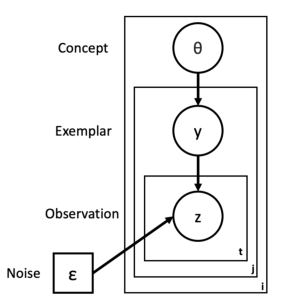
\includegraphics{figs/plate_diagram-1} 

}

\caption[Graphical representation of our model]{Graphical representation of our model. Circles indicate random variables. The squares indicate fixed model parameters.}\label{fig:plate_diagram}
\end{figure}
\end{CodeChunk}

\hypertarget{sampling}{%
\subsection{Sampling}\label{sampling}}

The formulation of the model as taking noisy samples from exemplars
allows us to do two things: First, we can explicitly model the learner's
decision on when to stop sampling by asking the model to decide, after
every sample \(z\), whether it wants to continue sampling from the same
stimulus or not. This is in contrast to the discrete time models
presented here and in previous work (Kidd et al., 2012; Poli et al.,
2020) , where we can only link information-theoretic measures to looking
data, but not provide a mechanism for how these measures could control
moment-to-moment sampling decisions. Second, a consequence of making a
decision at every time step is that we can study the behavior of another
information-theoretic measure: the expected information gain (EIG). EIG
is commonly used in rational analyses of information-seeking behavior -
that is to assess whether information-seeking is optimal with respect to
the learning task (Markant \& Gureckis, 2012; Oaksford \& Chater, 1994).
Importantly, EIG is a forward-looking measure that considers the
potential for learning from the next sample. Since discrete time models
operate on the level of a whole stimulus, rather than a series of
incomplete, noisy individual samples, EIG would look forward to the next
stimulus in these models, rather than to the next sample, and therefore
not be able to capture the decision of whether to keep looking. EIG to
describe looking time is therefore only possible in models with
temporally extended perception

We compute EIG by weighing the information gain from each possible next
observation by the probability of that observation. We defined
information gain as the KL-divergence between the hypothetical posterior
after observing a future sample \(z_{t+1}\) and the current posterior:
\begin{eqnarray}
EIG(z_{t+1}) = \sum_{z_{t+1} \in [0,1]} p(z_{t+1}|\theta_t) * D_{KL}(\theta_{t+1} || p(\theta_t))
\end{eqnarray} Finally, to get actual sampling behavior from the model,
it has to convert EIG into a binary decision about whether to continue
looking at the current sample, or to advance to the next trial. The
model does so using a Luce choice between the EIG from the next sample
and a constant EIG from looking away. \begin{eqnarray}
p(look) = \frac{EIG(z_{t+1})}{EIG(z_{t+1})+EIG(world)}
\end{eqnarray}

\hypertarget{alternative-linking-hypotheses}{%
\subsection{Alternative linking
hypotheses}\label{alternative-linking-hypotheses}}

We also studied the behavior of RANCH when replacing EIG with two other
linking hypotheses, surprisal and Kullback-Leibler (KL) divergence, used
in previous attempts to model infant looking behavior (Kidd et al.,
2012; Poli et al., 2020). These metrics have also been used to
approximate EIG in reinforcement learning literature (Kim, Sano, De
Freitas, Haber, \& Yamins, 2020). Surprisal, which we calculated as
\(-log(p(z|\theta))\), intuitively refers to how surprising an
observation \(z\) is given the model's beliefs about \(\theta\) - the
intuition that surprising events should result in longer looking times
has served as a foundational assumption in developmental psychology.
KL-divergence measures how much a model needs to change to accommodate a
new observation \(z\), and describes a distance between the model before
and after an observation. If an observation causes a large change, a
proportionally long looking time might be necessary to integrate the new
information. Formally, it describes a distance between the posterior
\(p(\theta_t)\) and the prior \(p(\theta_{t-1})\), computed as
\(\sum_{x \in X}{p(\theta = x|y)\frac{p(\theta_{t-1})}{p(\theta = t)}}\).
Unlike EIG, these alternative linking hypotheses are not strictly
maximizing information gain but provide psychologically plausible
heuristics with which to approximate EIG, given that they are
computationally much less intensive since there is no need to iterate
through all possible future samples \(z_{t+1}\) as in Eq. 4.

\hypertarget{experiment}{%
\section{Experiment}\label{experiment}}

To evaluate how well these models can explain looking time changes, we
developed a stimuli set and an experimental paradigm to reproduce the
key looking time patterns in adult participants. There are two
advantages to evaluating models with adult looking time data: 1) it is
relatively easy to acquire adult looking time data to reach sufficient
power; 2) adult looking time data can speak to the developmental
endpoints of the principles guiding looking time behaviors.

\hypertarget{methods}{%
\subsection{Methods}\label{methods}}

\hypertarget{stimuli}{%
\subsubsection{Stimuli}\label{stimuli}}

\begin{CodeChunk}
\begin{figure}[h]

{\centering 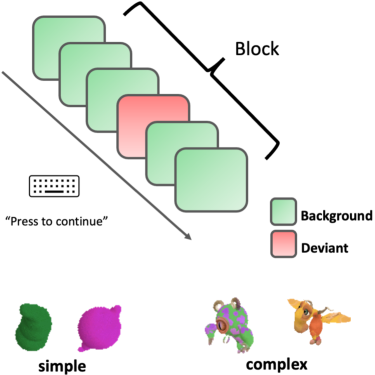
\includegraphics{figs/experimental_design-1} 

}

\caption[Experimental design and examples of simple and complex stimuli]{Experimental design and examples of simple and complex stimuli. In each block, a deviant could appear on the second, fourth (as depicted here) or sixth trial or not at all. Stimuli within a block were either all simple or all complex.}\label{fig:experimental_design}
\end{figure}
\end{CodeChunk}

We created the animated creatures using Spore (a game developed by Maxis
in 2008). There were forty creatures in total, half of which have low
perceptual complexity (e.g.~the creatures do not have limbs, additional
body parts, facial features, or textured skin), and half of which have
high perceptual complexity (i.e.~they do have the aforementioned
features; see Fig 2 for examples). We used the ``animated avatar''
function in Spore to capture the creatures in motion.

\hypertarget{procedure}{%
\subsubsection{Procedure}\label{procedure}}

The experiment was a web-based, self-paced visual presentation task.
Participants were instructed to look at a sequence of animated creatures
at their own pace and answer some questions throughout. On each trial,
an animated creature showed up on the screen. Participants could press
the down arrow to go to the next trial whenever they wanted to, after a
minimum viewing time of 500 ms.

Each block consisted of six trials. Unbeknownst to the participants,
each trial was either a background trial (B) or a deviant trial (D). A
background trial presented a creature repeatedly, and the deviant trial
presented a different creature from the background trial in the block.
Two creatures in the blocks were matched for visual complexity. There
were four sequences of background trials and deviant trials. Each
sequence appeared twice, once with high complexity stimuli and once with
low complexity stimuli. The deviant trial could appear at either the
second (BDBBBB), the fourth (BBBDBB), or the sixth trial (BBBBBD) in the
block. Two blocks did not have deviant trials (BBBBBB). The creatures
presented in the deviant trials and background trials were matched for
complexity. Each participant saw eight blocks in total, half of which
used creatures with high perceptual complexity, and half of which used
creatures with low perceptual complexity.

To test whether behavior was related to task demands, participants were
randomly assigned to one of three attention check conditions, differing
in the type of questions asked following each block: Curiosity, Memory,
and Math. In the Curiosity condition, participants were asked to rate
``How curious are you about the creature?'' on a 5-point Likert scale.
In the Memory condition, a forced-choice recognition question followed
each block (``Have you seen this creature before?''). The creature used
in the question in both conditions was either a creature presented in
the preceding block or a novel creature matched in complexity. In the
Math condition, the participants were asked a simple arithmetic question
(``What is 5 + 7?'') in a multiple-choice format.

At the end of the eight blocks, participants were asked to rate the
similarity between pairs of creatures and complexity of creatures they
encountered on a 7-point Likert scale. We used responses to these
questions to make sure our complexity manipulation was successful.

\hypertarget{participants}{%
\subsubsection{Participants}\label{participants}}

We recruited 449 participants (Age \emph{M} = 30.83; \emph{SD} = 17.44)
on Prolific. They were randomly assigned to one of the three conditions
of the experiment (Curiosity: \emph{N} = 156; Memory: \emph{N} = 137;
Math: \emph{N} = 156). Participants were excluded if they showed
irregular reaction times or their responses in the filler tasks
indicates low engagement with the experiment. All exclusion criteria
were pre-registered. The final sample included 380 participants.

\hypertarget{results}{%
\subsection{Results}\label{results}}

The sample size, methods, and main analyses were all pre-registered and
are available at {[}LINK{]}. Data and analysis scripts are available at
{[}LINK{]}. We first checked the basic complexity manipulations were
successful. Complex animated creatures were rated as more perceptually
complex (M = ; SD = ) than the simple animated creatures (M = ; SD = ).

Three criteria were selected to evaluate whether the paradigms
successfully captured the characteristic looking time patterns observed
in infant literature: habituation (the decrease in looking time for a
stimulus with repeated presentations), dishabituation (the increase in
looking time to a new stimulus after habituated to one stimulus), and
complexity effect (longer looking time for perceptually more complex
stimuli). The visualization of our results suggests that we reproduce
the phenomena qualitatively (Fig. 3, row1).To evaluate the phenomenon
quantitatively, we ran a linear mixed effects model with maximal random
effect structure. The predictors included in the model were a three-way
interaction term between the trial number (modeled as an exponential
decay; Keil 1991), the type of trial (background vs.~deviant) and the
complexity of the stimuli (simple vs.~complex). The model failed to
converge, so we pruned the model following the pre-registered procedure.
The final model included per-subject random intercepts. All predictors
except for the three-way interaction were significant from the model
(all \emph{t} \textless{} .001), providing a quantitative confirmation
that our paradigm successfully captured the key looking time patterns.

\hypertarget{model-comparison}{%
\section{Model comparison}\label{model-comparison}}

To evaluate whether RANCH can provide sufficient explanation of the
behavioral results, we simulated each model on the behavioral
experiment. Then, we searched for the best set of parameters that
yielded the highest Pearson's correlation between the model results and
behavioral results. We then compared the model fits within each model's
different linking hypotheses.

\hypertarget{model-experiment}{%
\subsection{Model experiment}\label{model-experiment}}

To model the behavioral experiment, we first represented the stimuli as
binary-valued vectors indicating the presence (1) or absence (0) of each
feature. All stimuli vectors were chosen to be length 6 to provide
sufficient representational flexibility. Complex stimuli were
represented as having three 1s and simple stimuli were represented as
having one 1, with the rest of the elements 0s. Individual stimuli are
then assembled into sequences to reflect the stimuli sequences in the
behavioral experiment. We ran four types of sequences, differing in the
position of the deviant: The sequence could either be a pure habituation
sequence with six background stimuli, or a deviant deviant appeared at
positions 2, 4 or 6. For a particular sequence, we constructed the
deviant stimulus based on the background stimulus to make sure that they
were always maximally different and had the same number of features
present.

The model then chose how to sample based on the three
information-theoretic linking hypotheses (EIG, surprisal and KL), as
well as the baseline linking hypotheses (random looking and no noise).

We let the model run 500 times for each sequence to obtain a reasonably
precise estimate of the model's behavior.

\hypertarget{parameter-estimation}{%
\subsection{Parameter estimation}\label{parameter-estimation}}

We performed an iterative grid search in parameter space for each
linking hypothesis. We a priori constrained our parameter space on the
prior beta distribution to have shape parameters
\(\alpha_{\theta} > \beta_{\theta}\), which describe the prior beliefs
as ``more likely to see the absence of a feature than the presence of a
feature.'' We then searched for the priors over the concept
(\(\theta\)), the noise parameter that decides how likely a feature
would be misperceived (\(\epsilon\)), and the constant EIG from the
world (\(EIG(world)\)). The prior over the noise parameter was fixed for
all searches (\(\alpha_{\epsilon}\) = 1;\(\beta_{\epsilon}\) = 10). We
selected the parameters that achieved the highest correlation with the
behavioral data (EIG: \(\alpha_{\theta}\) = 1, \(\beta_{\theta}\) = 4,
\(\epsilon\) = 0.065, \(EIG(world)\) = 0.01; KL: \(\alpha_{\theta}\) =
1, \(\beta_{\theta}\) = 5, \(\epsilon\) = 0.055, \(EIG(world)\) = 0.006;
Surprisal: \(\alpha_{\theta}\) = 1, \(\beta_{\theta}\) = 3, \(\epsilon\)
= 0.07, \(EIG(world)\) = 8).

\hypertarget{baseline-comparison}{%
\subsection{Baseline Comparison}\label{baseline-comparison}}

We next wanted to test what the effects are of removing two crucial
aspects of this model: 1) Making sampling choices based on learning from
samples, and 2) that perception is noisy. We implemented two lesioned
baseline models to which to contrast these information-theoretic linking
hypotheses. The first baseline model made totally random sampling
decisions by drawing \(p(look)\) from a uniform distribution between 0
and 1 at every time step. The second baseline model omitted the noisy
sampling aspect of RANCH and instead assumed that learning is free from
perceptual noise, i.e.~that learners can observe the exemplars \(y\)
directly. To do so, we set \(\epsilon\) to 0 and replaced the learner's
prior over \(\epsilon\) with a point mass at 0.000001 for numerical
stability. The baseline models used the parameters obtained from fitting
the EIG model to the behavioral data.

\begin{CodeChunk}
\begin{figure*}[h]

{\centering 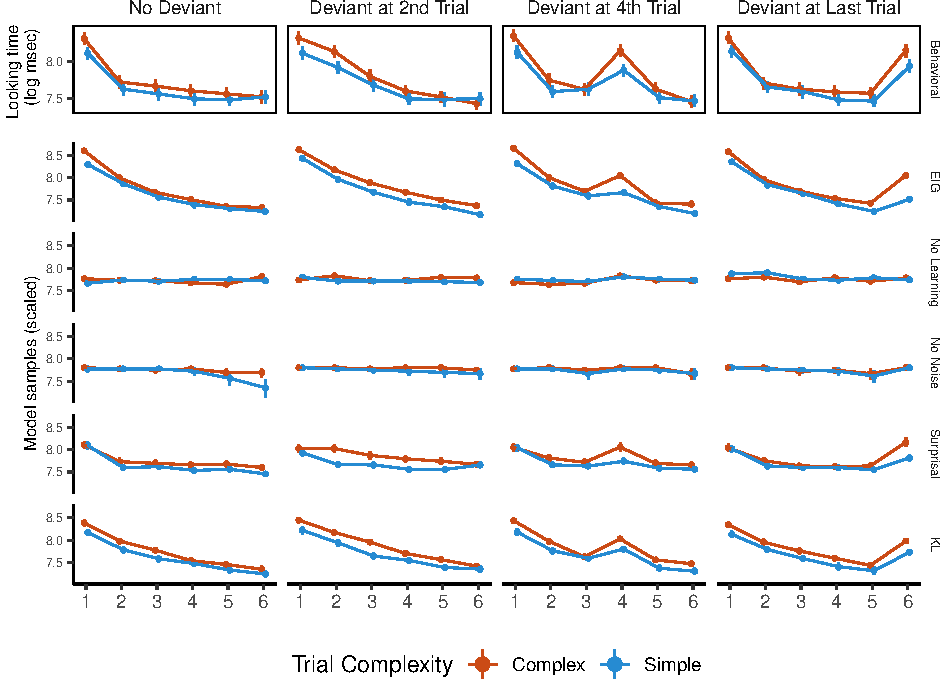
\includegraphics{figs/experiment_res-1} 

}

\caption[Continuous time model using different linking hypotheses provide qualitatively indistinguishable fits to the behavioral data]{Continuous time model using different linking hypotheses provide qualitatively indistinguishable fits to the behavioral data. All model results are log-transformed and adjusted to be at the same scale and intercepts as the log-transformed behavioral data. The solid lines represent human data, and the dotted lines represent the model's results. Red lines indicated results for complex stimuli, and blue lines indicated results for simple stimuli.}\label{fig:experiment_res}
\end{figure*}
\end{CodeChunk}

\hypertarget{results-1}{%
\subsection{Results}\label{results-1}}

RANCH reproduced the behavioral phenomena qualitatively, showing
habituation, dishabituation, and complexity effects (Fig. 3, row 2-4).
To quantitatively explore the model, we fit the models' output to the
behavioral data. All models' results were adjusted to match behavioral
data's scale and intercepts for easier comparisons. We found that the
three linking hypotheses were qualitatively indistinguishable in their
correlation to the behavioral data. Furthermore, the baseline models
performed far worse than RANCH using information-theoretic linking
hypotheses (see Table 1 for all computed metrics).

\hypertarget{discussion}{%
\subsection{Discussion}\label{discussion}}

The model results show that under RANCH's model architecture, the
performance of surprisal and KL can match that of EIG, a metric that can
quantitatively characterize the optimal exploratory behaviors in humans
(Coenen, Nelson, \& Gureckis, 2019; Oaksford \& Chater, 1994).To
calculate EIG one needs to consider all possible combinations of
features for the next observation, which becomes computationally
expensive and therefore psychologically implausible for naturalistic
stimuli, which may be expected to have a large number of features. The
proximity of model fits between EIG, KL, and surprisal suggests that
easier-to-compute metrics can be viable heuristics to which to anchor
sampling behavior.

The poor fit of the baseline models (Fig 3., row 5-6) further show that
both the learning model and the noisy sampling component of RANCH are
critical for modeling our phenomena of interest and provide good
quantitative fit to the data.

\hypertarget{general-discussion}{%
\section{General discussion}\label{general-discussion}}

The current work aimed to provide a computational model that can explain
the three key phenomena observed in typical infant looking time
paradigms: habituation, dishabituation, and complexity effect. RANCH
assumes a rational learner that takes noisy perceptual samples from
stimuli and makes sampling decisions based on expected information gain.
We evaluated the model with adult looking time data collected from a
paradigm that mirrors classic infant looking time paradigms. We found
that RANCH can successfully reproduce the patterns observed in
behavioral data. We find that other information theoretic quantities
(e.g.~KL-divergence and Surprisal) are good proxies for the rational
learning policy. Moreover, by contrasting the model results with our
baseline models, we showed that habituation, dishabituation, and
complexity effects only arise in a learning model that takes into
account the noisy nature of perception.

RANCH constitutes a significant step forward in the modeling of looking
time in that it models the moment-to-moment decision making process of
whether to keep sampling or look away. This is in contrast to previous
approaches, which incremented time in steps of whole stimuli, and
therefore can merely correlate information-theoretic variability in the
stimulus sequence to looking time. Our mechanistic account of the
sampling process depended on assuming that perception is noisy, which
made it necessary to take multiple samples from a stimulus until the
information content of the stimulus has been learned. The
moment-to-moment increments in which RANCH operates also enabled us to
use EIG as a linking hypothesis between learning and sampling. Using EIG
allowed us to perform the rational analysis of human behavior in our
paradigm, and contrast it with easier-to-compute and psychologically
plausible linking hypothesis, surprisal and KL.

There are several limitations to our work. For our behavioral data, one
concern is that our self-paced visual presentation task might not be
capturing participants' intrinsic interests in exploring the stimuli.
Adults may be viewing the stimuli in preparation for tasks, which
deviates from the infant looking duration primarily driven by intrinsic
motivation. However, across our three conditions with different filler
tasks, we found no differences in looking time patterns. This suggests
that the recorded behaviors are independent of task demand and are
likely tapping into the same processes that produce infants' looking
time patterns.

In regards to the model, a few concerns can be raised about the current
implementation. First of all, the current stimulus representation is
rather oversimplified. The stimuli are represented as a collection of
binary features. We did not take into consideration how perceptual
features can be processed with different priorities. Our complex stimuli
are different from simple stimuli not only in the number of perceptual
features but also in the kinds of features, such as eyes. There are
studies showing that features like eyes might be particularly
interesting to viewers because they convey potential social information
and serve as strong cues for animacy (Anderson, Meagher, Welder, \&
Graham, 2018; Birmingham, Bischof, \& Kingstone, 2009). Properly
representing different cognitive consequences of different types of
features could be an interesting next step for the model. In addition,
RANCH assumes that looking duration is determined by the decision
between ``continue looking'' and ``look away.'' However, one can argue
that in the behavioral experiment the participants were deciding between
``continuing looking at the current stimulus'' and ``looking at the next
stimulus.'' Building in these more sophisticated assumptions into the
model would certainly help us better understand looking time under a
rational analysis framework. But as a first step, our current work
suggests that a simple rational learner that takes noisy samples from a
set of independent binary features is capable of explaining key
phenomena in looking time change.

Our ultimate goal is to provide a rational learner model that can
account for information seeking behaviors through the lens of infants'
looking time. Here we have shown that such a model can reproduce adults'
looking time changes. As we further elaborate on our modeling approach,
our ongoing work with infants will eventually help address the
developmental trajectories of the mechanisms through which learners
decide what to look at, and when to stop looking.

\hypertarget{references}{%
\section{References}\label{references}}

\setlength{\parindent}{-0.1in} 
\setlength{\leftskip}{0.125in}

\noindent

\hypertarget{refs}{}
\begin{CSLReferences}{1}{0}
\leavevmode\vadjust pre{\hypertarget{ref-anderson2018animacy}{}}%
Anderson, N., Meagher, K., Welder, A., \& Graham, S. A. (2018). Animacy
cues facilitate 10-month-olds' categorization of novel objects with
similar insides. \emph{PloS One}, \emph{13}(11), e0207800.

\leavevmode\vadjust pre{\hypertarget{ref-aslin2007s}{}}%
Aslin, R. N. (2007). What's in a look? \emph{Developmental Science},
\emph{10}(1), 48--53.

\leavevmode\vadjust pre{\hypertarget{ref-birmingham2009saliency}{}}%
Birmingham, E., Bischof, W. F., \& Kingstone, A. (2009). Saliency does
not account for fixations to eyes within social scenes. \emph{Vision
Research}, \emph{49}(24), 2992--3000.

\leavevmode\vadjust pre{\hypertarget{ref-bitzer2014perceptual}{}}%
Bitzer, S., Park, H., Blankenburg, F., \& Kiebel, S. J. (2014).
Perceptual decision making: Drift-diffusion model is equivalent to a
bayesian model. \emph{Frontiers in Human Neuroscience}, \emph{8}, 102.

\leavevmode\vadjust pre{\hypertarget{ref-callaway2021fixation}{}}%
Callaway, F., Rangel, A., \& Griffiths, T. L. (2021). Fixation patterns
in simple choice reflect optimal information sampling. \emph{PLoS
Computational Biology}, \emph{17}(3), e1008863.

\leavevmode\vadjust pre{\hypertarget{ref-coenen2019asking}{}}%
Coenen, A., Nelson, J. D., \& Gureckis, T. M. (2019). Asking the right
questions about the psychology of human inquiry: Nine open challenges.
\emph{Psychonomic Bulletin \& Review}, \emph{26}(5), 1548--1587.

\leavevmode\vadjust pre{\hypertarget{ref-goodman2008rational}{}}%
Goodman, N. D., Tenenbaum, J. B., Feldman, J., \& Griffiths, T. L.
(2008). A rational analysis of rule-based concept learning.
\emph{Cognitive Science}, \emph{32}(1), 108--154.

\leavevmode\vadjust pre{\hypertarget{ref-haber2018learning}{}}%
Haber, N., Mrowca, D., Fei-Fei, L., \& Yamins, D. L. (2018). Learning to
play with intrinsically-motivated self-aware agents. \emph{arXiv
Preprint arXiv:1802.07442}.

\leavevmode\vadjust pre{\hypertarget{ref-hills2008search}{}}%
Hills, T. T., Todd, P. M., \& Goldstone, R. L. (2008). Search in
external and internal spaces: Evidence for generalized cognitive search
processes. \emph{Psychological Science}, \emph{19}(8), 802--808.

\leavevmode\vadjust pre{\hypertarget{ref-hunter1988multifactor}{}}%
Hunter, M. A., \& Ames, E. W. (1988). A multifactor model of infant
preferences for novel and familiar stimuli. \emph{Advances in Infancy
Research}.

\leavevmode\vadjust pre{\hypertarget{ref-hunter1983effects}{}}%
Hunter, M. A., Ames, E. W., \& Koopman, R. (1983). Effects of stimulus
complexity and familiarization time on infant preferences for novel and
familiar stimuli. \emph{Developmental Psychology}, \emph{19}(3), 338.

\leavevmode\vadjust pre{\hypertarget{ref-kersten2004object}{}}%
Kersten, D., Mamassian, P., \& Yuille, A. (2004). Object perception as
bayesian inference. \emph{Annu. Rev. Psychol.}, \emph{55}, 271--304.

\leavevmode\vadjust pre{\hypertarget{ref-kidd2012goldilocks}{}}%
Kidd, C., Piantadosi, S. T., \& Aslin, R. N. (2012). The goldilocks
effect: Human infants allocate attention to visual sequences that are
neither too simple nor too complex. \emph{PloS One}, \emph{7}(5),
e36399.

\leavevmode\vadjust pre{\hypertarget{ref-kim2020active}{}}%
Kim, K., Sano, M., De Freitas, J., Haber, N., \& Yamins, D. (2020).
Active world model learning with progress curiosity. In
\emph{International conference on machine learning} (pp. 5306--5315).
PMLR.

\leavevmode\vadjust pre{\hypertarget{ref-liquin2021developmental}{}}%
Liquin, E. G., Callaway, F., \& Lombrozo, T. (2021). Developmental
change in what elicits curiosity. In \emph{Proceedings of the annual
meeting of the cognitive science society} (Vol. 43).

\leavevmode\vadjust pre{\hypertarget{ref-markant2012does}{}}%
Markant, D., \& Gureckis, T. (2012). Does the utility of information
influence sampling behavior? In \emph{Proceedings of the annual meeting
of the cognitive science society} (Vol. 34).

\leavevmode\vadjust pre{\hypertarget{ref-oaksford1994rational}{}}%
Oaksford, M., \& Chater, N. (1994). A rational analysis of the selection
task as optimal data selection. \emph{Psychological Review},
\emph{101}(4), 608.

\leavevmode\vadjust pre{\hypertarget{ref-oudeyer2007intrinsic}{}}%
Oudeyer, P.-Y., Kaplan, F., \& Hafner, V. V. (2007). Intrinsic
motivation systems for autonomous mental development. \emph{IEEE
Transactions on Evolutionary Computation}, \emph{11}(2), 265--286.

\leavevmode\vadjust pre{\hypertarget{ref-paulus2022should}{}}%
Paulus, M. (2022). Should infant psychology rely on the
violation-of-expectation method? Not anymore. \emph{Infant and Child
Development}, e2306.

\leavevmode\vadjust pre{\hypertarget{ref-pirolli1999information}{}}%
Pirolli, P., \& Card, S. (1999). Information foraging.
\emph{Psychological Review}, \emph{106}(4), 643.

\leavevmode\vadjust pre{\hypertarget{ref-poli2020infants}{}}%
Poli, F., Serino, G., Mars, R., \& Hunnius, S. (2020). Infants tailor
their attention to maximize learning. \emph{Science Advances},
\emph{6}(39), eabb5053.

\leavevmode\vadjust pre{\hypertarget{ref-raz2020learning}{}}%
Raz, G., \& Saxe, R. (2020). Learning in infancy is active, endogenously
motivated, and depends on the prefrontal cortices. \emph{Annual Review
of Developmental Psychology}, \emph{2}, 247--268.

\leavevmode\vadjust pre{\hypertarget{ref-sim2019another}{}}%
Sim, Z. L., \& Xu, F. (2019). Another look at looking time: Surprise as
rational statistical inference. \emph{Topics in Cognitive Science},
\emph{11}(1), 154--163.

\leavevmode\vadjust pre{\hypertarget{ref-smith2018developing}{}}%
Smith, L. B., Jayaraman, S., Clerkin, E., \& Yu, C. (2018). The
developing infant creates a curriculum for statistical learning.
\emph{Trends in Cognitive Sciences}, \emph{22}(4), 325--336.

\leavevmode\vadjust pre{\hypertarget{ref-tafreshi2014analysis}{}}%
Tafreshi, D., Thompson, J. J., \& Racine, T. P. (2014). An analysis of
the conceptual foundations of the infant preferential looking paradigm.
\emph{Human Development}, \emph{57}(4), 222--240.

\leavevmode\vadjust pre{\hypertarget{ref-tenenbaum1999bayesian}{}}%
Tenenbaum, J. B. (1999). Bayesian modeling of human concept learning.
\emph{Advances in Neural Information Processing Systems}, 59--68.

\end{CSLReferences}

\bibliographystyle{apacite}


\end{document}
